\documentclass[tikz,border=10pt]{standalone}
\usepackage{tikz}
\begin{document}
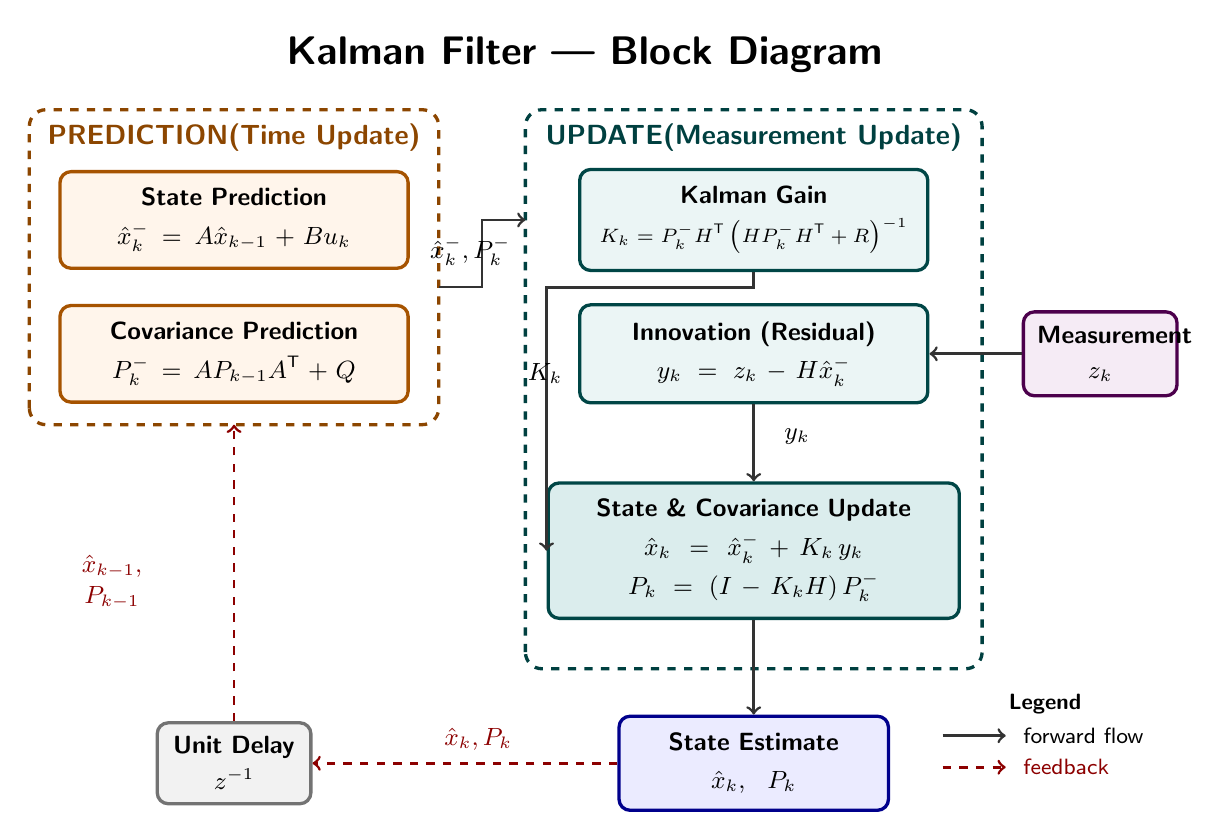
\begin{tikzpicture}[
  every node/.style={font=\sffamily},
  predictbox/.style={rectangle,draw=orange!65!black,very thick,rounded corners=4pt,
    fill=orange!8,align=center,text width=4.0cm,inner sep=6pt,font=\sffamily\small},
  updatebox/.style={rectangle,draw=teal!55!black,very thick,rounded corners=4pt,
    fill=teal!8,align=center,text width=4.0cm,inner sep=6pt,font=\sffamily\small},
  finalbox/.style={rectangle,draw=teal!55!black,very thick,rounded corners=4pt,
    fill=teal!14,align=center,text width=4.8cm,inner sep=6pt,font=\sffamily\small},
  measbox/.style={rectangle,draw=violet!60!black,very thick,rounded corners=4pt,
    fill=violet!8,align=center,text width=1.6cm,inner sep=5pt,font=\sffamily\small},
  statebox/.style={rectangle,draw=blue!55!black,very thick,rounded corners=4pt,
    fill=blue!8,align=center,text width=3.0cm,inner sep=6pt,font=\sffamily\small},
  delaybox/.style={rectangle,draw=black!55,very thick,rounded corners=4pt,
    fill=black!5,align=center,text width=1.6cm,inner sep=5pt,font=\sffamily\small},
  fwdarrow/.style={->,very thick,black!80,line width=1pt},
  fbarrow/.style={->,very thick,dashed,red!55!black,line width=1pt},
]

% ---------- Title ----------
\node[font=\sffamily\Large\bfseries] at (7.35,10.4) {Kalman Filter --- Block Diagram};

% ---------- Prediction container ----------
\draw[draw=orange!55!black,dashed,very thick,rounded corners=6pt] (0.3,5.7) rectangle (5.5,9.7);
\node[font=\sffamily\bfseries,text=orange!55!black] at (2.9,9.35) {PREDICTION\\(Time Update)};

\node[predictbox] (P1) at (2.9,8.3) {\textbf{State Prediction}\\[3pt]$\hat{x}_k^{-}=A\hat{x}_{k-1}+Bu_k$};
\node[predictbox] (P2) at (2.9,6.6) {\textbf{Covariance Prediction}\\[3pt]$P_k^{-}=AP_{k-1}A^{\mathsf T}+Q$};

% ---------- Update container ----------
\draw[draw=teal!50!black,dashed,very thick,rounded corners=6pt] (6.6,2.6) rectangle (12.4,9.7);
\node[font=\sffamily\bfseries,text=teal!50!black] at (9.5,9.35) {UPDATE\\(Measurement Update)};

\node[updatebox] (U1) at (9.5,8.3) {\textbf{Kalman Gain}\\[3pt]{\scriptsize$K_k=P_k^{-}H^{\mathsf T}\left(HP_k^{-}H^{\mathsf T}+R\right)^{-1}$}};
\node[updatebox] (U2) at (9.5,6.6) {\textbf{Innovation (Residual)}\\[3pt]$y_k=z_k-H\hat{x}_k^{-}$};
\node[finalbox]  (U3) at (9.5,4.1) {\textbf{State \& Covariance Update}\\[3pt]$\hat{x}_k=\hat{x}_k^{-}+K_k\,y_k$\\[3pt]$P_k=(I-K_kH)\,P_k^{-}$};

% ---------- Measurement input ----------
\node[measbox] (MEAS) at (13.9,6.6) {\textbf{Measurement}\\[2pt]$z_k$};

% ---------- State estimate output ----------
\node[statebox] (SE) at (9.5,1.4) {\textbf{State Estimate}\\[3pt]$\hat{x}_k,\;P_k$};

% ---------- Unit delay (feedback path) ----------
\node[delaybox] (DL) at (2.9,1.4) {\textbf{Unit Delay}\\[2pt]$z^{-1}$};

% ---------- Forward flow arrows ----------
\draw[fwdarrow] (5.5,7.45) -- (6.05,7.45) -- (6.05,8.3) -- (6.6,8.3);
\node[font=\sffamily\small] at (5.9,7.9) {$\hat{x}_k^{-},P_k^{-}$};

\draw[fwdarrow] (U1.south) -- ++(0,-0.2) -| (U3.west);
\node[font=\sffamily\small] at (6.85,6.35) {$K_k$};

\draw[fwdarrow] (U2.south) -- (U3.north);
\node[font=\sffamily\small] at (10.05,5.55) {$y_k$};

\draw[fwdarrow] (MEAS.west) -- (U2.east);

\draw[fwdarrow] (U3.south) -- (SE.north);

% ---------- Feedback arrows ----------
\draw[fbarrow] (SE.west) -- (DL.east);
\node[font=\sffamily\small,text=red!55!black] at (6.0,1.7) {$\hat{x}_k,P_k$};

\draw[fbarrow] (DL.north) -- (2.9,5.7);
\node[font=\sffamily\small,align=center,text=red!55!black] at (1.35,3.7) {$\hat{x}_{k-1},$\\$P_{k-1}$};

% ---------- Legend ----------
\node[font=\sffamily\footnotesize\bfseries] at (13.2,2.15) {Legend};
\draw[fwdarrow] (11.9,1.75) -- (12.7,1.75);
\node[font=\sffamily\footnotesize,anchor=west] at (12.8,1.75) {forward flow};
\draw[fbarrow] (11.9,1.35) -- (12.7,1.35);
\node[font=\sffamily\footnotesize,anchor=west,text=red!55!black] at (12.8,1.35) {feedback};

\end{tikzpicture}
\end{document}
